\section{Evaluation Methodology and Channel Models}
\label{sec:channels}

Every number in this report was measured on one of six channels, and
the channels differ in kind: three are simulations of increasing
physical fidelity, one is two circuit boards joined by a wire, one is a
software-defined radio at 7\,MHz, and one is a family of host-side
harnesses that reproduce a specific board failure without the boards.
Each was chosen because it answers a question the others cannot, and
several findings in later sections turn on knowing which channel a
figure came from --- a sensitivity measured on the article channel does
not transfer to the wire stand, and a loss rate measured on the wire
stand says nothing about fading.  This section defines the channels
once, states the statistical conventions every sweep shares, and ends
with a table (Table~\ref{tab:channels}) that maps each headline result
of the report to the channel it was measured on.

\subsection{Conventions}
\label{sec:conventions}

\paragraph{SNR.}  Unless a section says otherwise, SNR follows the
source article's convention: total signal power against total noise
power in the full 6\,kHz Nyquist band of the 12\,kHz-sampled audio.
The waveform occupies only $\approx$2.1\,kHz (300--2400\,Hz), so the
same operating point reads $\approx$4.5\,dB higher against in-band
noise only, and $\approx$3.8\,dB higher in the ham-standard 2.5\,kHz
convention ($-17.9$\,dB here is $\approx-14.1$\,dB ham).  Two
measurements in Part~\ref{part:impl} use a different reference and say
so where they do: the ZC-anchor A/B of Section~\ref{sec:zcscan}
references the transmitted waveform's full-band RMS (about 9\,dB
pessimistic against this convention), and the boards' own integer SNR
estimator reports through the output map of
Section~\ref{sec:cport_snrcal}, calibrated so that it reads what the
float estimator reads on the same waveform.

\paragraph{Sensitivity.}  The sensitivity of a configuration is the
lowest SNR at which its packet error rate is at most 10\,\%, read off a
PER waterfall swept in 0.5\,dB steps.  Sensitivities are quoted for
the recalibrated receiver (Section~\ref{sec:llr}) except where the
article reproduction itself is the subject.

\paragraph{Trials.}  The article-reproduction curves use 120 packets
per point; the rate ladder 48; the calibration and code-family
studies 300 (binomial uncertainty $\le\pm3$\,\% near a waterfall
midpoint); the streaming study 300 bursts $=$ 6\,000 blocks; smaller
counts (20--40) are stated inline where they occur and carry the
uncertainty they imply.  Every A/B comparison draws \emph{paired}
channel realizations --- the same seed, hence the same noise, offset
and fade, in both arms --- so that the difference between arms is the
treatment and not the draw.  Every figure has a generating script in
\texttt{experiments/} and a JSON record beside the PNG in
\texttt{results/}; non-default trial counts get suffixed filenames so a
smoke run cannot overwrite a reference sweep.

\subsection{The Article Channel (Audio Domain)}
\label{sec:chan_article}

\texttt{ofdm\_phy/channel.py} is the source article's air-channel
simulator, reproduced parameter for parameter, and it drives every
PHY-layer sweep of Part~\ref{part:phy} and most link-layer experiments.
It operates on the 12\,kHz real audio waveform and applies, in order:

\begin{table}[H]
    \centering
    \caption{The article channel model (\texttt{simulate\_channel}).}
    \label{tab:chan_article}
    \small
    \begin{tabular}{@{}lp{9.4cm}@{}}
    \toprule
    \textbf{Impairment} & \textbf{Model} \\
    \midrule
    Timing offset & the frame is prepended with $t_0$ samples of
        silence; $t_0$ is drawn per trial (below) \\
    Carrier offset & the analytic signal is rotated by
        $f_0 + 5\,\mathrm{Hz}\cdot(t/T)^2$: a constant offset plus a
        quadratic drift reaching $+5$\,Hz at the end of the frame \\
    Rayleigh fading & optional; a complex Gaussian gain band-limited by
        a second-order Butterworth at the Doppler frequency
        (0.1--0.5\,Hz is typical HF QSB), normalized to unit mean power,
        applied to the analytic signal before the real part is taken \\
    Multipath & real FIR $[1,\,0,\,0.4,\,0,\,0,\,0.2]$ at 12\,kHz
        (taps at 0, 167 and 417\,$\mu$s) \\
    AWGN & Gaussian noise sized from the \emph{mean} power of the
        faded, convolved signal to the nominal SNR, so under fading the
        instantaneous SNR swings about the nominal \\
    BSC & block phase inversion: each 160-sample block (13.3\,ms) is
        multiplied by $-1$ with probability $10^{-3}$ \\
    BEC & block erasure: each 160-sample block is zeroed with
        probability $2\cdot10^{-2}$ \\
    \bottomrule
    \end{tabular}
\end{table}

The BSC and BEC terms are the article's abstraction of impulsive
interference and deep, brief fades: they act on 13.3\,ms blocks of the
\emph{waveform}, not on bits, and a single erasure removes a third of a
NORMAL OFDM symbol.  They are on in every sweep that calls the channel
with its defaults; the fading term is off by default and switched on
where a section says so (the broadcast group-size study of
Section~\ref{sec:bcgroup} at 0.5\,Hz, the fading RF demonstrations).

What a sweep draws per trial varies with its purpose, and the
differences matter when comparing figures across sections:

\begin{table}[H]
    \centering
    \caption{Per-trial draws on the article channel, by experiment.}
    \label{tab:chan_draws}
    \footnotesize
    \begin{tabular}{@{}p{5.6cm}llr@{}}
    \toprule
    \textbf{Experiment} & \textbf{Timing offset} & \textbf{CFO $f_0$} &
        \textbf{Trials/pt} \\
    \midrule
    Article reproduction (\texttt{ber\_per\_simulation}) &
        $\mathcal{U}[200, 1500)$ & $\mathcal{U}(-100, +100)$\,Hz & 120 \\
    Rate ladder (\texttt{ladder\_sweep}) &
        $\mathcal{U}[200, 1500)$ & $\mathcal{U}(-100, +100)$\,Hz & 48 \\
    Adaptive modes (\texttt{adaptive\_modes}) &
        $\mathcal{U}[200, 1500)$ & $\mathcal{U}(-100, +100)$\,Hz & 48 \\
    LLR calibration and code studies &
        $\mathcal{U}[300, 1200)$ & $\mathcal{U}(-60, +60)$\,Hz & 300 \\
    STF vs.\ Newman detection A/B (\texttt{stf\_vs\_newman}) &
        $\mathcal{U}[200, 1500)$ & $\mathcal{U}(-300, +300)$\,Hz & 150 \\
    Streaming, broadcast studies & fixed 300 & fixed $+3.0$\,Hz &
        20--300 \\
    \bottomrule
    \end{tabular}
\end{table}

The streaming and broadcast studies fix the offset and CFO on purpose:
they measure the link layer's behaviour over long waveforms, and a
random CFO per trial would confound the synchronizer's contribution
with the transport's.  The two-lag unwrap of
Section~\ref{sec:cfo_unwrap} is the one place the choice of CFO turned
out to be load-bearing: the integer detector's defect appears only
within a few hertz of a coarse-bin boundary, $+3.0$\,Hz is next to one,
and so the broadcast studies at that fixed offset were the experiments
that surfaced it --- a random CFO per trial would have diluted it to a
few percent and hidden it.  Sweeping the offset across one bin then
located it.

\subsection{The SSB RF Chain and Oscillator Model}
\label{sec:rf}

The article channel injects the carrier offset as a parameter.  The RF
layer (\texttt{ofdm\_phy/rf.py}) instead models the transceiver chain
an audio modem actually sits in, so that carrier offsets \emph{emerge
from oscillator physics}: two stations with realistic reference
oscillators produce whatever audio-band CFO their ppm errors and
thermal drifts imply, and the AFC loop of Section~\ref{sec:afc} has
something physical to net.  It is the channel of the recorded
two-station demonstrations (Section~\ref{sec:results}) and of the AFC
measurements.

\subsubsection{The SSB Chain}

Simulation runs at a 48\,kHz IF rate with a 12\,kHz carrier standing in
for the RF carrier; LO errors are specified in ppm of the nominal RF
frequency (e.g.\ 7.1\,MHz), so audio-band offsets come out physically
correct (Figure~\ref{fig:rf_chain}).  The channel between the USB
modulator and the product detector carries the same impairments as the
article channel --- fading, multipath, AWGN, BSC/BEC --- applied at the
IF rate.

\begin{figure}[H]
    \centering
    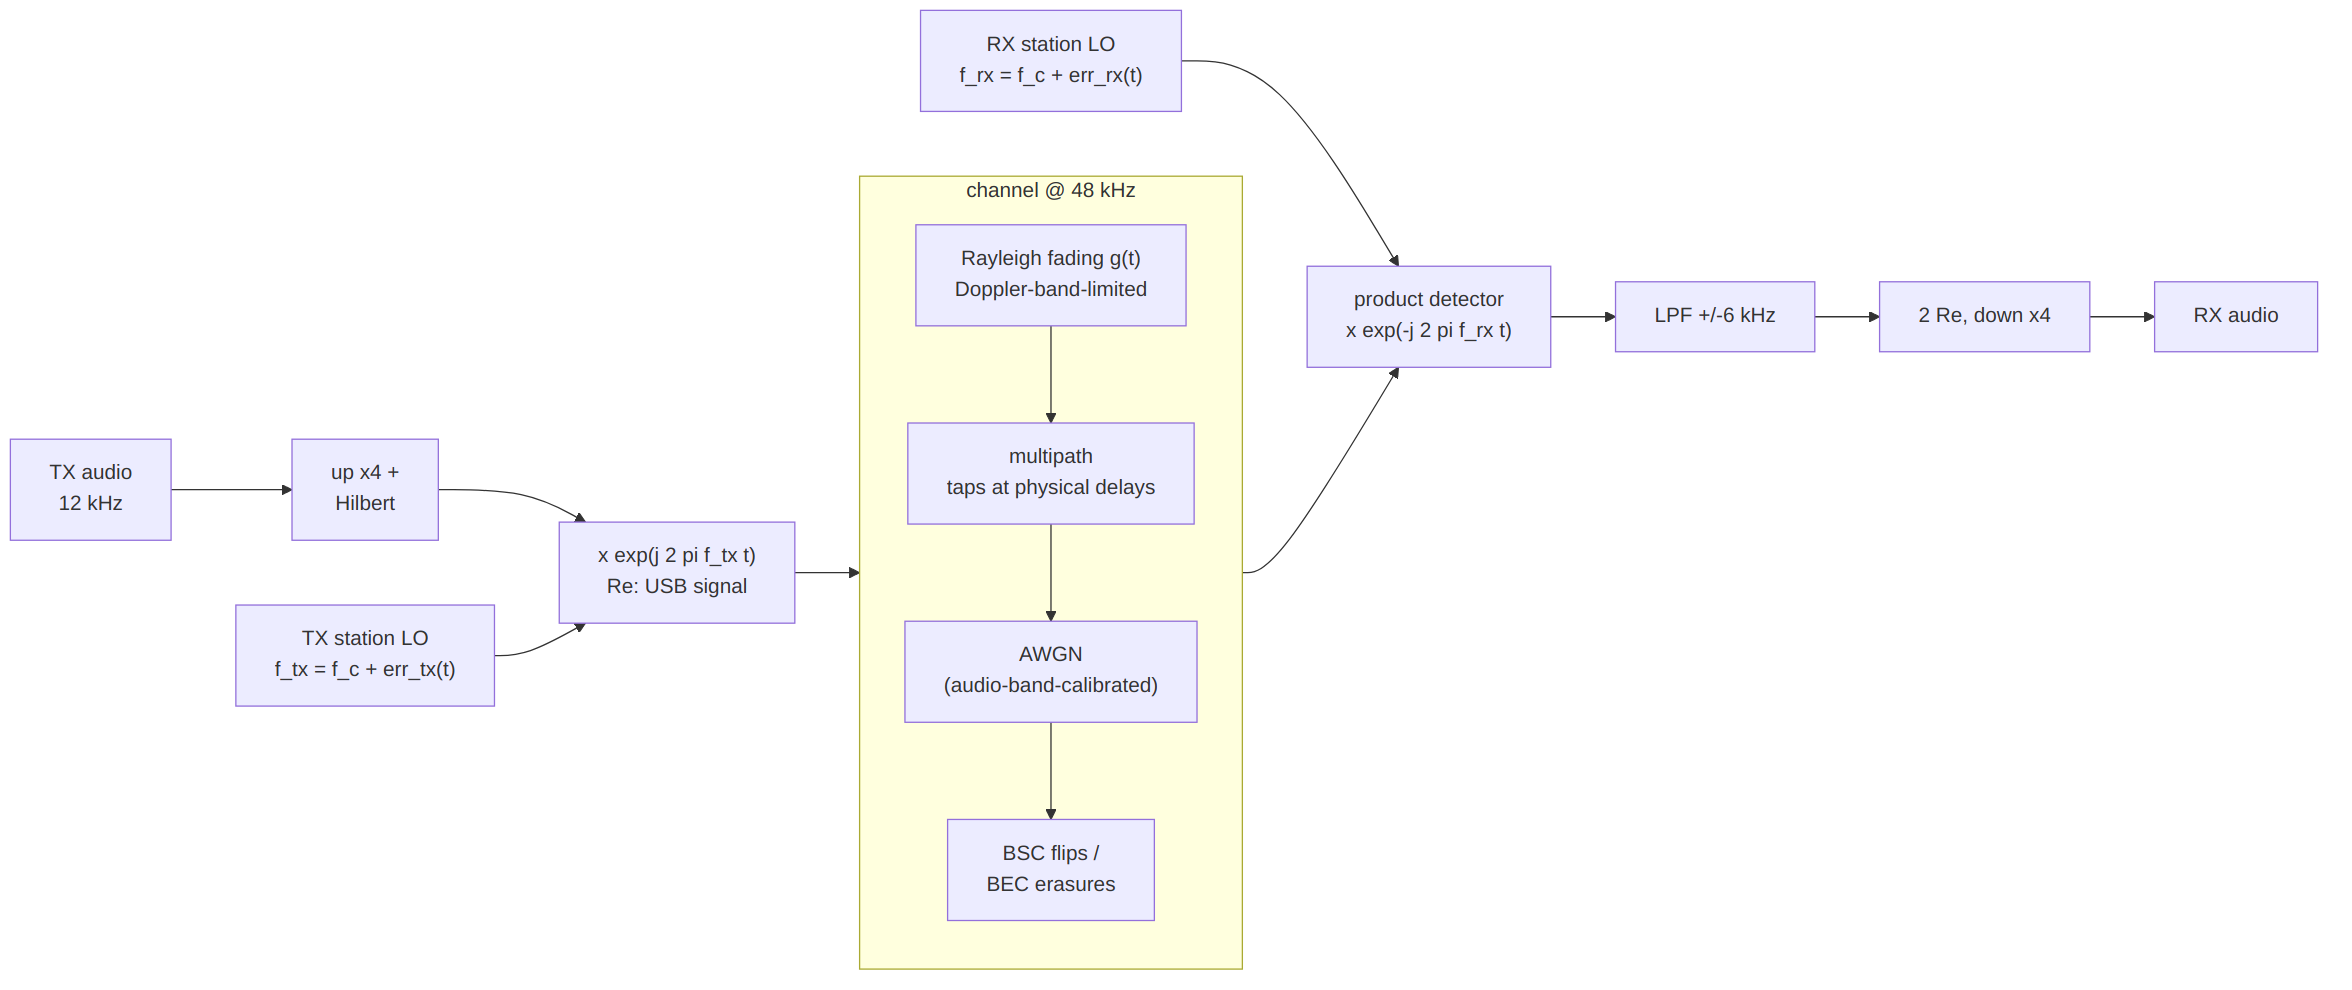
\includegraphics[width=\textwidth]{images/rf_chain.png}
    \caption{The RF chain: USB modulator, 48\,kHz channel (fading,
             multipath, AWGN, BSC/BEC), product detector.}
    \label{fig:rf_chain}
\end{figure}

\subsubsection{The LO Model}

Each \texttt{StationRF} has \emph{one} reference oscillator shared by
its TX and RX, as in a real transceiver:
\[
    \mathrm{err}(t) \;=\; f_{\mathrm{rf}} \cdot \mathrm{ppm} \cdot
    10^{-6} \;+\; \mathrm{drift}_{\mathrm{Hz/s}} \cdot t \;+\;
    \mathrm{trim}_{\mathrm{Hz}},
\]
and the audio CFO between two stations is
$\mathrm{err}_{tx}(t) - \mathrm{err}_{rx}(t)$
(Figure~\ref{fig:lo_model}).  Validated against the modem's own CFO
measurements to 0.1\,Hz at $+99.4$, $-106.5$, and $+284.0$\,Hz
scenarios.  \texttt{trim\_hz} is the AFC hook of
Section~\ref{sec:afc}.  The scenarios used in this report: the recorded
demonstration runs station~A at $+6$\,ppm and B at $-8$\,ppm on
7.1\,MHz (A$\to$B CFO $\approx+99.4$\,Hz) with a passive monitor at
$+2$\,ppm; the AFC scenarios run two worn-TCXO rigs on 14.2\,MHz
starting $+284$\,Hz apart with opposing thermal drifts (0.09\,Hz/s
relative).

\begin{figure}[H]
    \centering
    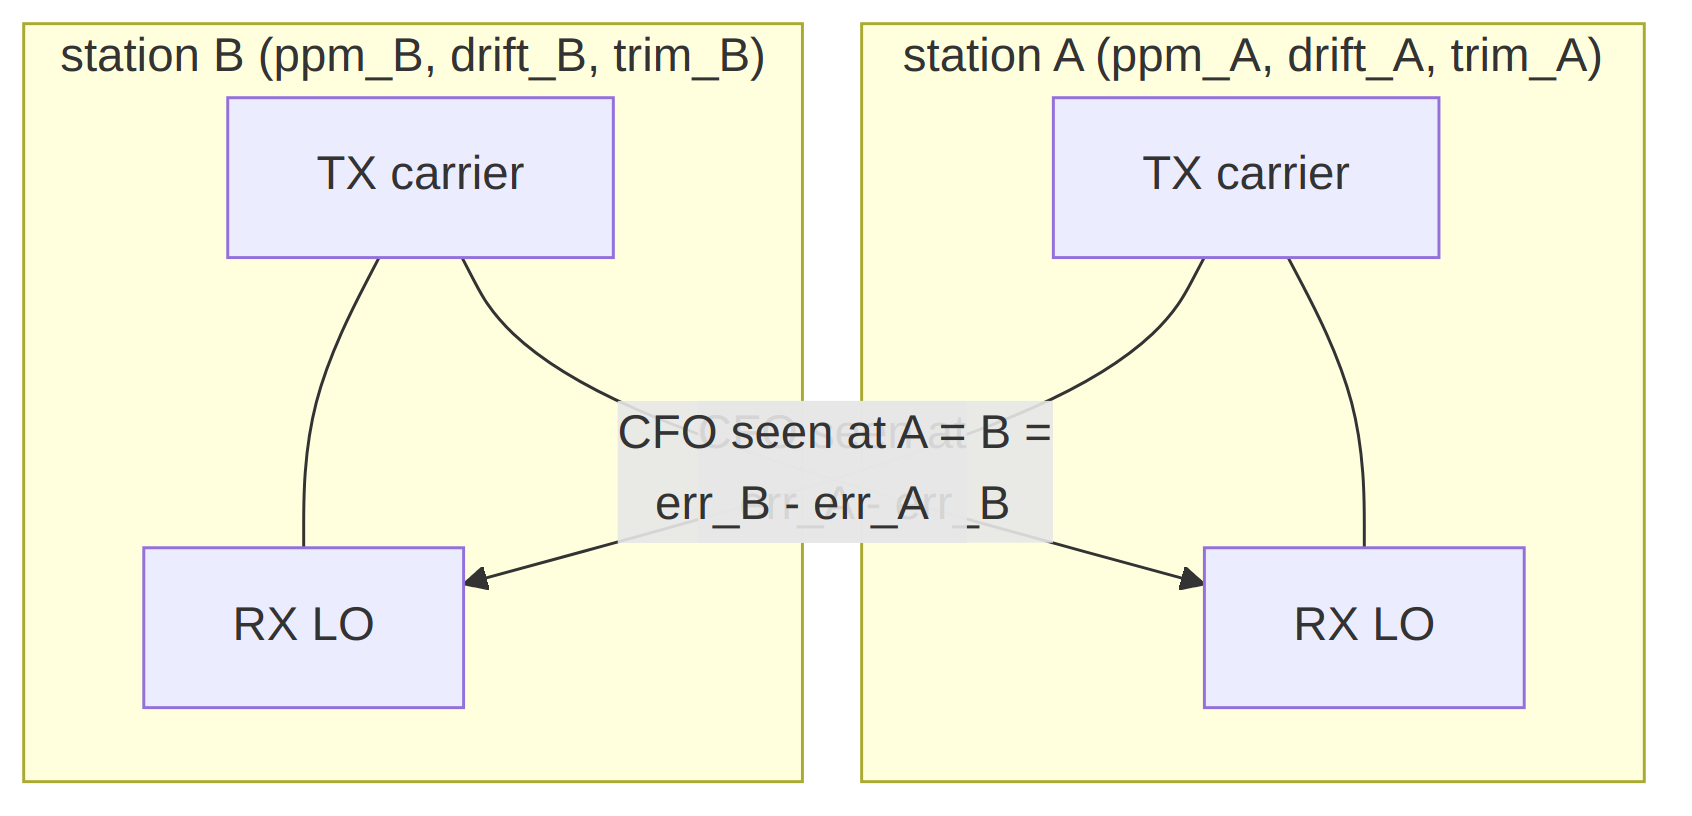
\includegraphics[width=0.75\textwidth]{images/lo_model.png}
    \caption{Per-station shared-reference LO model: where CFO comes
             from.}
    \label{fig:lo_model}
\end{figure}

\subsubsection{Calibration Subtleties}

Three traps are documented in code comments because each silently
costs dB if gotten wrong:

\begin{itemize}
    \item \textbf{AWGN sizing.}  The product detector's
          $\mathrm{Re}(\cdot)$ halves \emph{uncorrelated noise} power
          but not the coherent signal, so the RF noise variance factor
          is $2 \cdot P_{\mathrm{sig}} \cdot 10^{-\mathrm{SNR}/10}$
          --- not the naive bandwidth ratio, which is 3\,dB off.  With
          the correct factor the audio-band SNR convention matches the
          audio-domain simulator, so all measured sensitivities carry
          over (9/10 decodes at $-5$\,dB through the full RF chain).
    \item \textbf{Rayleigh fading.}  Complex Gaussian band-limited to
          the Doppler bandwidth (0.1--0.5\,Hz, typical HF QSB), unit
          mean power, applied to the analytic signal; AWGN is sized
          from the \emph{average} faded power, so instantaneous SNR
          swings around the nominal value.
    \item \textbf{Multipath at RF.}  The audio-domain tap delays are
          physical, so taps map to interpolation-factor-spaced
          positions at the RF rate.
\end{itemize}

\subsection{The Virtual Channel Daemon}
\label{sec:chan_virtual}

The demonstration applications of Section~\ref{sec:cport_demo} do not
call a channel function; they talk to \emph{devices}.
\texttt{demoapp/driver.py} exposes two station devices and one
configuration device over Unix sockets and moves 12\,kHz int16 audio
between them in 10\,ms ticks (120 samples), applying per direction:

\begin{itemize}
    \item a propagation \textbf{delay line} (\texttt{delay\_ms});
    \item \textbf{Rayleigh fading} as a streamed one-pole-filtered
          complex Gaussian gain at the Doppler corner
          (\texttt{fading\_hz}) --- a real-time approximation of the
          Butterworth fader above, chosen because it has no warm-up
          and no memory beyond one sample;
    \item \textbf{AWGN} sized against the \emph{tracked} RMS of the
          delivered signal (a $0.98/0.02$ tracker that updates only
          while a signal is present), so the nominal SNR holds across
          frames of different modes and levels;
    \item \textbf{half-duplex muting}: a station transmitting hears
          nothing, which is what gives the carrier-sense and
          reply-timer logic something to be wrong about.
\end{itemize}

The channel parameters can be changed while a session runs
(\texttt{demoapp/chanctl.py}), which is how mid-transfer fades are
produced.  A \emph{time scale} runs the whole exchange faster than
real time; it is what makes a 20-minute transfer a one-minute test,
with one caveat measured in Section~\ref{sec:rto}: protocol time is
sample-derived, so at $25\times$ on an eight-core host the decoding
side's clock lags the transmitting side's and timeouts appear that no
channel caused.  Drop the time scale to $8\times$ before believing a
timeout.  This is the channel of every ``virtual channel'' figure in
Sections~\ref{sec:link}, \ref{sec:broadcast} and~\ref{sec:cport}.

\subsection{The Two-Board Wire Stand}
\label{sec:chan_wire}

The first channel with no simulation in it: two STM32H743 boards, each
clocking its 12\,kHz converters from its own crystal and PLL, board~A's
DAC driving board~B's ADC (and B's driving A's) through one signal wire
and one ground wire, with an ESP32 JTAG probe daisy-chained through
both parts for the beacon that reports every counter without touching
the link (Section~\ref{sec:cport_twoboard}).  Its properties, all
measured:

\begin{table}[H]
    \centering
    \caption{The wire stand as a channel.}
    \label{tab:chan_wire}
    \small
    \begin{tabular}{@{}lp{8.6cm}@{}}
    \toprule
    \textbf{Property} & \textbf{Measured} \\
    \midrule
    Converters & 12-bit DAC at 3/4 of full scale, re-read by a 16-bit
        ADC; 2.472\,V pk-pk about a 1.643\,V mid-rail \\
    Clock offset & two independent crystals; bounded at $\pm56$\,ppm
        from a 54\,000-sample capture, and $\approx$5\,ppm from the
        $+0.01$\,Hz residual CFO the modem measures \\
    SNR & clean: $+16.2$\,dB on EXTREME frames, $+20.9\ldots+22.5$\,dB
        on NORMAL, $+24.7$\,dB reported by the calibrated estimator; it
        does not fade and cannot be attenuated in software \\
    DC & the operating point is whatever the peer's DAC parks at
        between frames --- up to 0.83\,V off mid-rail before the park
        fix, a constant $2.7\times10^{8}$ on the peer's carrier
        sense; now blocked at 7.5\,Hz before anything reads it
        (Section~\ref{sec:cport_harden}) \\
    Carrier sense levels & quiet wire $\approx2\times10^{4}$ mean
        square; a full-strength frame $1.1\times10^{8}$ \\
    Capture & one 2283\,ms blocking decode per EXTREME frame --- the
        figure that sizes every FIFO and host timeout in
        Sections~\ref{sec:radio} and~\ref{sec:host} \\
    \bottomrule
    \end{tabular}
\end{table}

The stand answers questions of a different kind from the simulations.
It cannot measure sensitivity --- there is no attenuator --- but it is
the only channel here with real converters, real clocks, a real DC
operating point and real half-duplex turnaround, and every defect in
Sections~\ref{sec:radio} and~\ref{sec:host} lived in one of those four.
Where a stand finding needed a channel the wire cannot produce (a
fade, an ADC that clips, a converter that sticks), the harnesses of
Section~\ref{sec:chan_harness} reproduced the board's impairments on
the host, and the wire then confirmed the fix.

\subsection{Impairment Harnesses on the Host}
\label{sec:chan_harness}

Five host-side harnesses in \texttt{cport/bench/} run the shipped C
code over channels that reproduce, or exceed, what the boards see.
They are regression gates (\texttt{make robust} runs the first four),
and each exists because a board failure needed a channel the wire
could not provide:

\begin{description}
    \item[\texttt{burst\_repro} (\texttt{make burstrepro}).]  The wire
        as an impairment set, applied one at a time or all at once:
        the 12-bit DAC at 3/4 scale re-read by the 16-bit ADC
        (\texttt{-q}); a sample-rate offset between the ends by linear
        interpolation, up to 56\,ppm; static DC to $\pm18\,000$\,LSB
        (\texttt{-dc}); DC steps; $2.5\times$ clipping into
        saturation; 50\,Hz hum at 8\,000\,LSB; impulse clicks; a
        converter stuck at its DC level for 8 samples 60 times a
        second; optionally the firmware's own DC blocker in the path.
        The abuse matrix of Table~\ref{tab:harden} is this harness.
    \item[\texttt{bc\_fade} (\texttt{make bcfade}).]  AWGN whose SNR
        follows a V-shaped profile in time: $+20$\,dB until 40\,s, a
        ramp down to the floor by 80\,s, the floor ($-5$\,dB by
        default, $-2$\,dB in the second run) until 140\,s, and a ramp
        back to $+20$\,dB by 180\,s.  It runs the firmware's broadcast
        block/statistics/re-rung machinery --- sender state machine,
        receiver walk and both control decisions --- on identical fades
        for a fixed-rung and an adaptive arm
        (Section~\ref{sec:bcfade}).
    \item[\texttt{bc\_soak} (\texttt{make bcsoak}).]  A clean channel
        with no noise at all, and the receiver's own timing as the
        only variable: two-frame broadcast groups of $\approx$30
        bytes, random payloads, random inter-group gaps, and a random
        sample-phase lead before each group, thousands of groups per
        run.  It reproduces the group loss of
        Section~\ref{sec:voice_onair} deterministically per seed and
        is the regression for the detector's commit gate.
    \item[\texttt{bc\_repro} (\texttt{make bcrepro}).]  The firmware's
        build-and-walk path for one broadcast group under the wire's
        requantization, at rung 4 and rung 0.
    \item[\texttt{zc\_anchor\_ab} (\texttt{make zcab}).]  Byte-identical
        EXTREME waveforms --- same seed, noise and carrier offset ---
        through two builds of the detector, 250 trials per point across
        the sensitivity knee plus 250 noise-only runs per arm.  Its SNR
        reference is the transmitted waveform's full-band RMS, about
        9\,dB pessimistic against the convention of
        Section~\ref{sec:conventions}.
\end{description}

Two further host runs belong in this list because they are the only
measurements of their kind: the noise-only false-alarm test of the
detection thresholds (0 false alarms in 20 runs per mode,
Section~\ref{sec:modes}, and 0 in 250 per arm in the ZC-anchor A/B),
and the carrier-sense scenario suite (\texttt{make cstest}: boot
latch, parked DC bare and through the blocker, 45-s busy hold,
frame/gap cycling, DC-step transient), which replays every measured
field failure of carrier sense as a scenario.

\subsection{The SDR Path}
\label{sec:chan_sdr}

The last channel is radio.  \texttt{demoapp/sdr\_driver.py} presents
the same socket devices as the virtual channel daemon but carries the
audio over SSB on a HackRF One at 2.4\,Msps, tuned to 7.000\,MHz
(Section~\ref{sec:cport_sdr}).  Three configurations were used, each a
figure in Section~\ref{sec:cport_sdr}:

\begin{itemize}
    \item \textbf{Loopback}, hardware-free: two stations cross-connected
          through the entire SSB chain in software --- Hilbert
          transform, interpolation to the SDR rate, \emph{int8
          quantization}, decimation and product detection.  The DSP
          regression test; it reproduces the SSB model of
          Section~\ref{sec:rf} sample by sample.
    \item \textbf{Instrumented}, with a tinySA Ultra on USB: as an
          analyser wired to the antenna port it measures the
          transmitted spectrum and the drive sweep; as a source, its
          calibration output (a reference tone at a nominal
          $-25$\,dBm) drives the receiver through a 40\,dB pad for the
          receive-chain calibration of Section~\ref{sec:link_budget_measured}
          (frequency error $-3.31$\,ppm, linearity 1.002\,dB/dB, noise
          floor $-95.5$\,dBm in 6\,kHz).
    \item \textbf{Off-air}: the radio is half duplex, so a second
          transmitter stands in --- a laptop sound card plays a
          generated file into an AM modulator on an external generator
          at 7.000\,MHz, into the SDR through a 40\,dB pad.  Detection
          is synchronous (carrier recovered), so the decoded CFO reads
          zero; the decoded SNRs were $+8.5$ to $+14.4$\,dB.  This is a
          real RF path but not a transmit-to-receive loop of the
          modem's own waveform generator, which wants a second radio.
\end{itemize}

\subsection{Which Result Was Measured Where}
\label{sec:chan_map}

\begin{table}[H]
    \centering
    \caption{Headline results and the channel each was measured on.}
    \label{tab:channels}
    \small
    \begin{tabular}{@{}p{7.4cm}p{6.6cm}@{}}
    \toprule
    \textbf{Result} & \textbf{Channel} \\
    \midrule
    Article reproduction, $-7.2$\,dB sensitivity, BER/PER curves
        (Sections~\ref{sec:sync}, \ref{sec:results}) &
        article channel, 120 trials/pt \\
    Mode sensitivities $-7.6/-11.7/-17.9$\,dB, the 13-rung ladder
        (Sections~\ref{sec:modes}, \ref{sec:link}) &
        article channel, 40--48 trials/pt \\
    LLR recalibration $+1.5$--2\,dB; LDPC vs.\ conv; 16-QAM studies
        (Sections~\ref{sec:llr}, \ref{sec:coding}) &
        article channel, 300 frames/pt, paired \\
    Streaming $1.73\times$ at 0.08\,dB; broadcast group-size study
        (Sections~\ref{sec:stream}, \ref{sec:bcgroup}) &
        article channel, fixed offset/CFO; fading 0.5\,Hz for the
        group-size study \\
    AFC netting $+284$\,Hz $\to$ $<12$\,Hz; recorded two-station
        demonstrations (Sections~\ref{sec:afc}, \ref{sec:results}) &
        SSB RF chain with the LO model \\
    Burst windows, file transfers, reply timer, broadcast sequence
        traces (Sections~\ref{sec:burstwin}, \ref{sec:rto},
        \ref{sec:broadcast_seq}) & virtual channel daemon \\
    Fixed-point parity, two-lag unwrap, coarse-search A/B
        (Section~\ref{sec:fixed}) & article channel, paired \\
    Processor and memory budgets (Section~\ref{sec:cport_ontarget}) &
        STM32H743 over JTAG, byte-identical data \\
    ZC-anchor cost and sensitivity bound
        (Section~\ref{sec:zcscan}) & \texttt{zc\_anchor\_ab} harness \\
    First frames, radio firmware, burst debugging, sentinel, SNR map,
        transfer levers (114\,B/s), operator ceilings
        (Sections~\ref{sec:radio}, \ref{sec:cport_caps}) &
        two-board wire stand \\
    DC-blind front end, carrier-sense hardening
        (Section~\ref{sec:cport_harden}) &
        \texttt{burst\_repro} abuse matrix, then the wire \\
    Broadcast block statistics and re-rung
        (Section~\ref{sec:cport_bcast}) & wire stand; adaptation under
        fade on \texttt{bc\_fade} \\
    KISS and IP tunnel throughput (Sections~\ref{sec:cport_kiss},
        \ref{sec:cport_iptun}) & wire stand \\
    Transmitted spectrum, drive sweep, receive-chain calibration,
        off-air decode (Section~\ref{sec:cport_sdr}) & SDR path \\
    Voice codec evaluation (Section~\ref{sec:cport_voice}) &
        no channel: host-side, codec in and out \\
    Voice on the air: profiles, latency, group loss and its fix
        (Section~\ref{sec:voice_onair}) & wire stand, then
        \texttt{bc\_soak} for the defect and the wire for the
        confirmation \\
    \bottomrule
    \end{tabular}
\end{table}
